\documentclass[onecolumn]{preport}
\usepackage[dvipdfmx]{graphicx}
\usepackage{listings}
\usepackage{color}
\usepackage{url}
\graphicspath{{figs/}}
\title{クラウド基盤ソフトウェア課題レポート}
\author{480206515 知能機械情報学専攻 河村洋一郎}

\begin{document}

\pagestyle{empty}
\maketitle
\thispagestyle{empty}
\sloppy

\section{実験設定}
\subsection{実験に用いた計算機}
実験は手元のラップトップPC(ThinkPad P52S)で行った。計算機のスペックは
\begin{table}[htb]
  \begin{tabular}{c|l} \hline
    CPU & Intel(R) Core(TM) i7-8650U CPU @ 1.90GHz, 4コア8スレッド \\ \hline
    メモリ & 32GB DDR4 \\ \hline
    グラフィックボード &  Quadro P500 Mobile \\ \hline
  \end{tabular}
\end{table}
である。
\subsection{CPU仮想化なしの環境}
仮想化を行わない場合のホストOSはLinux (Ubuntu 18.04)を用いた。詳細なカーネルの情報は以下である。
\lstset{
  basicstyle={\ttfamily},
  identifierstyle={\small},
  commentstyle={\smallitshape},
  keywordstyle={\small\bfseries},
  ndkeywordstyle={\small},
  stringstyle={\small\ttfamily},
  frame={tb},
  breaklines=true,
  columns=[l]{fullflexible},
  %% numbers=left,
  xrightmargin=0zw,
  xleftmargin=3zw,
  numberstyle={\scriptsize},
  stepnumber=1,
  numbersep=1zw,
  lineskip=-0.5ex}
\begin{lstlisting}[language=c]
uname -a
Linux capricorn 5.3.0-61-generic #55~18.04.1-Ubuntu SMP Mon Jun 22 16:40:20 UTC 2020 x86_64 x86_64 x86_64 GNU/Linux
\end{lstlisting}

\subsection{CPU仮想化ありの環境}
仮想化を行った場合のホストOSはWindows10、仮想化にはVirtualBoxを使用し、ゲストOSにはLinux (Ubuntu 18.04)を用いた。

\subsection{行った実験}
行った実験は以下の\textcolor{red}{hoge}個である。なお、今回は実験を行う途中に他のプロセスの優先度を変更したり止めることはせず、一般的なユースケースを想定してプログラムを実行した。
\begin {enumerate}
\item フィボナッチ数を求める処理.\\ 漸化式$F_{n+2} = F_{n+1} + F{n}$を用いて繰り返しで$F(n)$を求める$O(n)$の計算.同様の計算は10回行い平均と分散を求めた。
\item ローカルディスクにあるファイルへのread/write処理.\\ランダムな$N$文字をファイルに書き込み,その後書き込んだ文字を読み出す処理.同様の計算は10回行い平均と分散を求めた。
\item USBメモリにあるファイルへのread/write処理
\item OpenGLのbench mark (glmark2 \cite{glmark2})
\end {enumerate}

\section{結果}
\subsection{フィボナッチ数を求める処理}


\subsection{OpenGL}
ベンチマークの結果を以下に示す。
\begin{table}[htb]
  \begin{tabular}{c|c} \hline
    仮想化なし & 仮想化なし \\ \hline
    1149  & 32GB DDR4 \\ \hline
  \end{tabular}
\end{table}

詳細なベンチマークの結果は\ref{}に示す。

\section{考察}



%% 本稿はプログレスレポートのテンプレートである\cite{Sakai}.
%% 本稿における「、」や「。」は、\verb|make pub|を実行することで、「,」や「.」に変更される。
%% 図は\figref{nowprinting}や\tabref{sample}として参照する.
%% \begin{figure}[tbh]
%%  \begin{center}
%%   \begin{minipage}{0.3\columnwidth}
%%    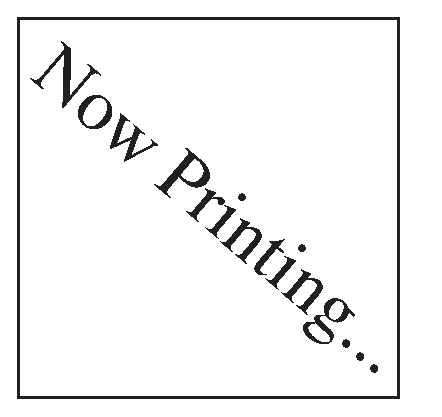
\includegraphics[width=\columnwidth]{nowprinting.eps}
%%    \caption{eps図の参考例}
%%   \end{minipage}
%%   \hspace{0.15\columnwidth}
%%   \begin{minipage}{0.3\columnwidth}
%%    
\includegraphics[width=\columnwidth]{dj.jpg}
%%    \caption{jpg図の参考例}
%%   \end{minipage}
%%   \label{figure:nowprinting}
%%  \end{center}
%% \end{figure}

%% \begin{table}[tbh]
%%  \begin{center}
%%   \begin{tabular}{|l|r|} \hline
%%   A1 & B1 \\
%%   A2 & B2 \\ \hline
%%   \end{tabular}
%%   \caption{図の参考例}
%%   \label{table:sample}
%%  \end{center}
%% \end{table}

\section{おわりに}

\section{付録}
\subsection{OpenGLのベンチマークのスコア詳細}
仮想化なし
\lstset{
  basicstyle={\ttfamily},
  identifierstyle={\small},
  commentstyle={\smallitshape},
  keywordstyle={\small\bfseries},
  ndkeywordstyle={\small},
  stringstyle={\small\ttfamily},
  frame={tb},
  breaklines=true,
  columns=[l]{fullflexible},
  %% numbers=left,
  xrightmargin=0zw,
  xleftmargin=3zw,
  numberstyle={\scriptsize},
  stepnumber=1,
  numbersep=1zw,
  lineskip=-0.5ex}
\begin{lstlisting}[language=c]

$ glmark2
=======================================================
    glmark2 2014.03+git20150611.fa71af2d
=======================================================
    OpenGL Information
    GL_VENDOR:     NVIDIA Corporation
    GL_RENDERER:   Quadro P500/PCIe/SSE2
    GL_VERSION:    4.6.0 NVIDIA 440.100
=======================================================
[build] use-vbo=false: FPS: 988 FrameTime: 1.012 ms
[build] use-vbo=true: FPS: 1481 FrameTime: 0.675 ms
[texture] texture-filter=nearest: FPS: 1419 FrameTime: 0.705 ms
[texture] texture-filter=linear: FPS: 1484 FrameTime: 0.674 ms
[texture] texture-filter=mipmap: FPS: 1580 FrameTime: 0.633 ms
[shading] shading=gouraud: FPS: 978 FrameTime: 1.022 ms
[shading] shading=blinn-phong-inf: FPS: 980 FrameTime: 1.020 ms
[shading] shading=phong: FPS: 920 FrameTime: 1.087 ms
[shading] shading=cel: FPS: 1110 FrameTime: 0.901 ms
[bump] bump-render=high-poly: FPS: 764 FrameTime: 1.309 ms
[bump] bump-render=normals: FPS: 1479 FrameTime: 0.676 ms
[bump] bump-render=height: FPS: 1703 FrameTime: 0.587 ms
[effect2d] kernel=0,1,0;1,-4,1;0,1,0;: FPS: 1384 FrameTime: 0.723 ms
[effect2d] kernel=1,1,1,1,1;1,1,1,1,1;1,1,1,1,1;: FPS: 980 FrameTime: 1.020 ms
[pulsar] light=false:quads=5:texture=false: FPS: 1496 FrameTime: 0.668 ms
[desktop] blur-radius=5:effect=blur:passes=1:separable=true:windows=4: FPS: 695 FrameTime: 1.439 ms
[desktop] effect=shadow:windows=4: FPS: 858 FrameTime: 1.166 ms
[buffer] columns=200:interleave=false:update-dispersion=0.9:update-fraction=0.5:update-method=map: FPS: 425 FrameTime: 2.353 ms
[buffer] columns=200:interleave=false:update-dispersion=0.9:update-fraction=0.5:update-method=subdata: FPS: 627 FrameTime: 1.595 ms
[buffer] columns=200:interleave=true:update-dispersion=0.9:update-fraction=0.5:update-method=map: FPS: 570 FrameTime: 1.754 ms
[ideas] speed=duration: FPS: 1643 FrameTime: 0.609 ms
[jellyfish] <default>: FPS: 783 FrameTime: 1.277 ms
[terrain] <default>: FPS: 106 FrameTime: 9.434 ms
[shadow] <default>: FPS: 1037 FrameTime: 0.964 ms
[refract] <default>: FPS: 145 FrameTime: 6.897 ms
[conditionals] fragment-steps=0:vertex-steps=0: FPS: 1522 FrameTime: 0.657 ms
[conditionals] fragment-steps=5:vertex-steps=0: FPS: 1548 FrameTime: 0.646 ms
[conditionals] fragment-steps=0:vertex-steps=5: FPS: 1619 FrameTime: 0.618 ms
[function] fragment-complexity=low:fragment-steps=5: FPS: 1585 FrameTime: 0.631 ms
[function] fragment-complexity=medium:fragment-steps=5: FPS: 1375 FrameTime: 0.727 ms
[loop] fragment-loop=false:fragment-steps=5:vertex-steps=5: FPS: 1545 FrameTime: 0.647 ms
[loop] fragment-steps=5:fragment-uniform=false:vertex-steps=5: FPS: 1595 FrameTime: 0.627 ms
[loop] fragment-steps=5:fragment-uniform=true:vertex-steps=5: FPS: 1513 FrameTime: 0.661 ms
=======================================================
                                  glmark2 Score: 1149
=======================================================
\end{lstlisting}


\bibliographystyle{junsrt}
\bibliography{p-report}

\end{document}
